\section{Results}
\label{sec:result}
\subsection{RQ1. Change patterns}
\label{sec:result:pattern}


%The taxonomy includes change of lock type, change of lock variable, synchronization addition, synchronization removal, lock release, volatile addition, volatile removal, class replacement, thread-safe class replacement, thread management, thread status management,

%\begin{table*}
%\zhong{Please delete this table.}
%	\centering
%	\caption{Taxonomy}
%	\begin{tabular}{|c|c|c|}\hline
%		Type&Example&Occurrence\\\hline
%		Changing lock type&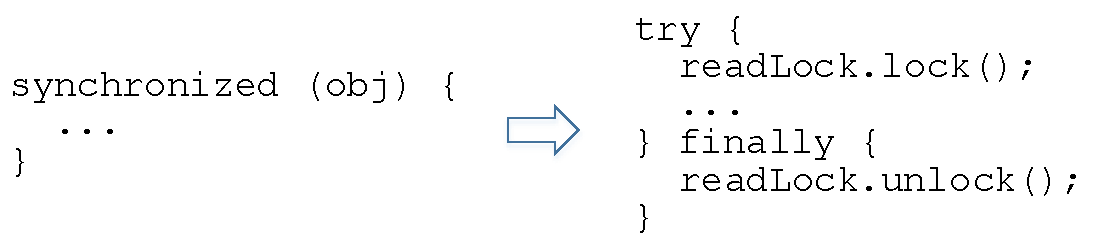
\includegraphics[scale=0.35]{pattern1}&4\\\hline
%		Changing lock instance&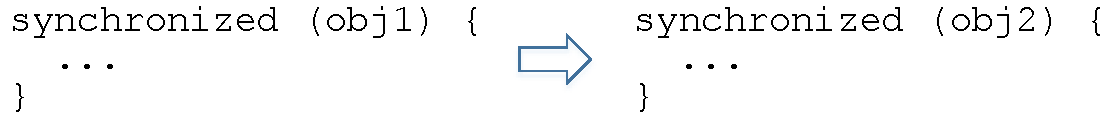
\includegraphics[scale=0.35]{pattern2}&6\\\hline
%		Changing critical section&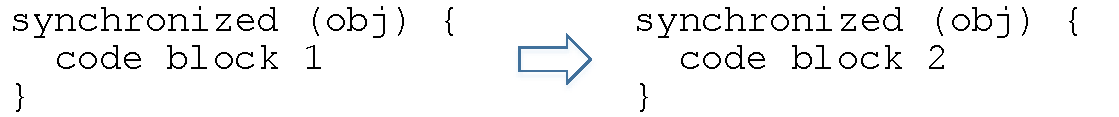
\includegraphics[scale=0.35]{pattern3}&35\\\hline
%		Adding or removing \texttt{volatile}&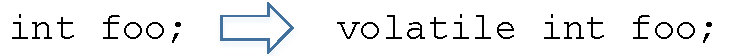
\includegraphics[scale=0.35]{pattern4}&47\\\hline
%		Thread-safe class replacement&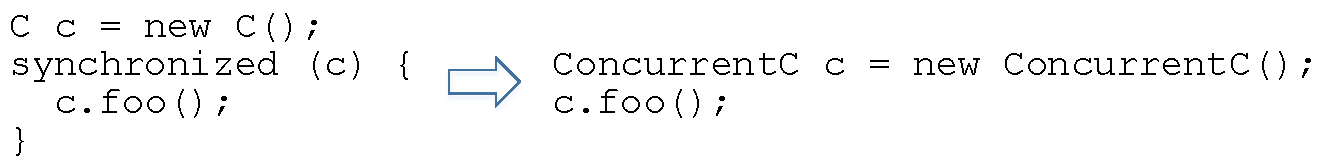
\includegraphics[scale=0.35]{pattern5}&32\\\hline
%		Thread management&&\\\hline
%		%Other class replacement&Some other concurrent related class replacement&\\\hline
%	\end{tabular}
%\end{table*}

%Switch to another type of lock
%Switch to another lock instace
%Change critical sections, which are protected by synchronization
%Add or remove 'volatile' modifier of a class field
%Use thread-safe class instead of handling concurrency control manually

%Table~\ref{} and \ref{} show an overview of our extracted change patterns. \zhong{Please explain the columns.}

Table~\ref{table:patterns} and table~\ref{table:patterns2} show an overview of our extracted change patterns. The first column is the sequence number of patterns. The ``source'' column shows the concrete examples of patterns. We put related source code in it. The left is the original code and the right is the modified code. We align the corresponding statements. We use different colors to mark modified lines. The ``pattern'' column shows the extracted patterns. They are short as they ignore the specific statements.

\begin{table*}
	\centering
\caption{Change patterns}\vspace*{-3ex}
	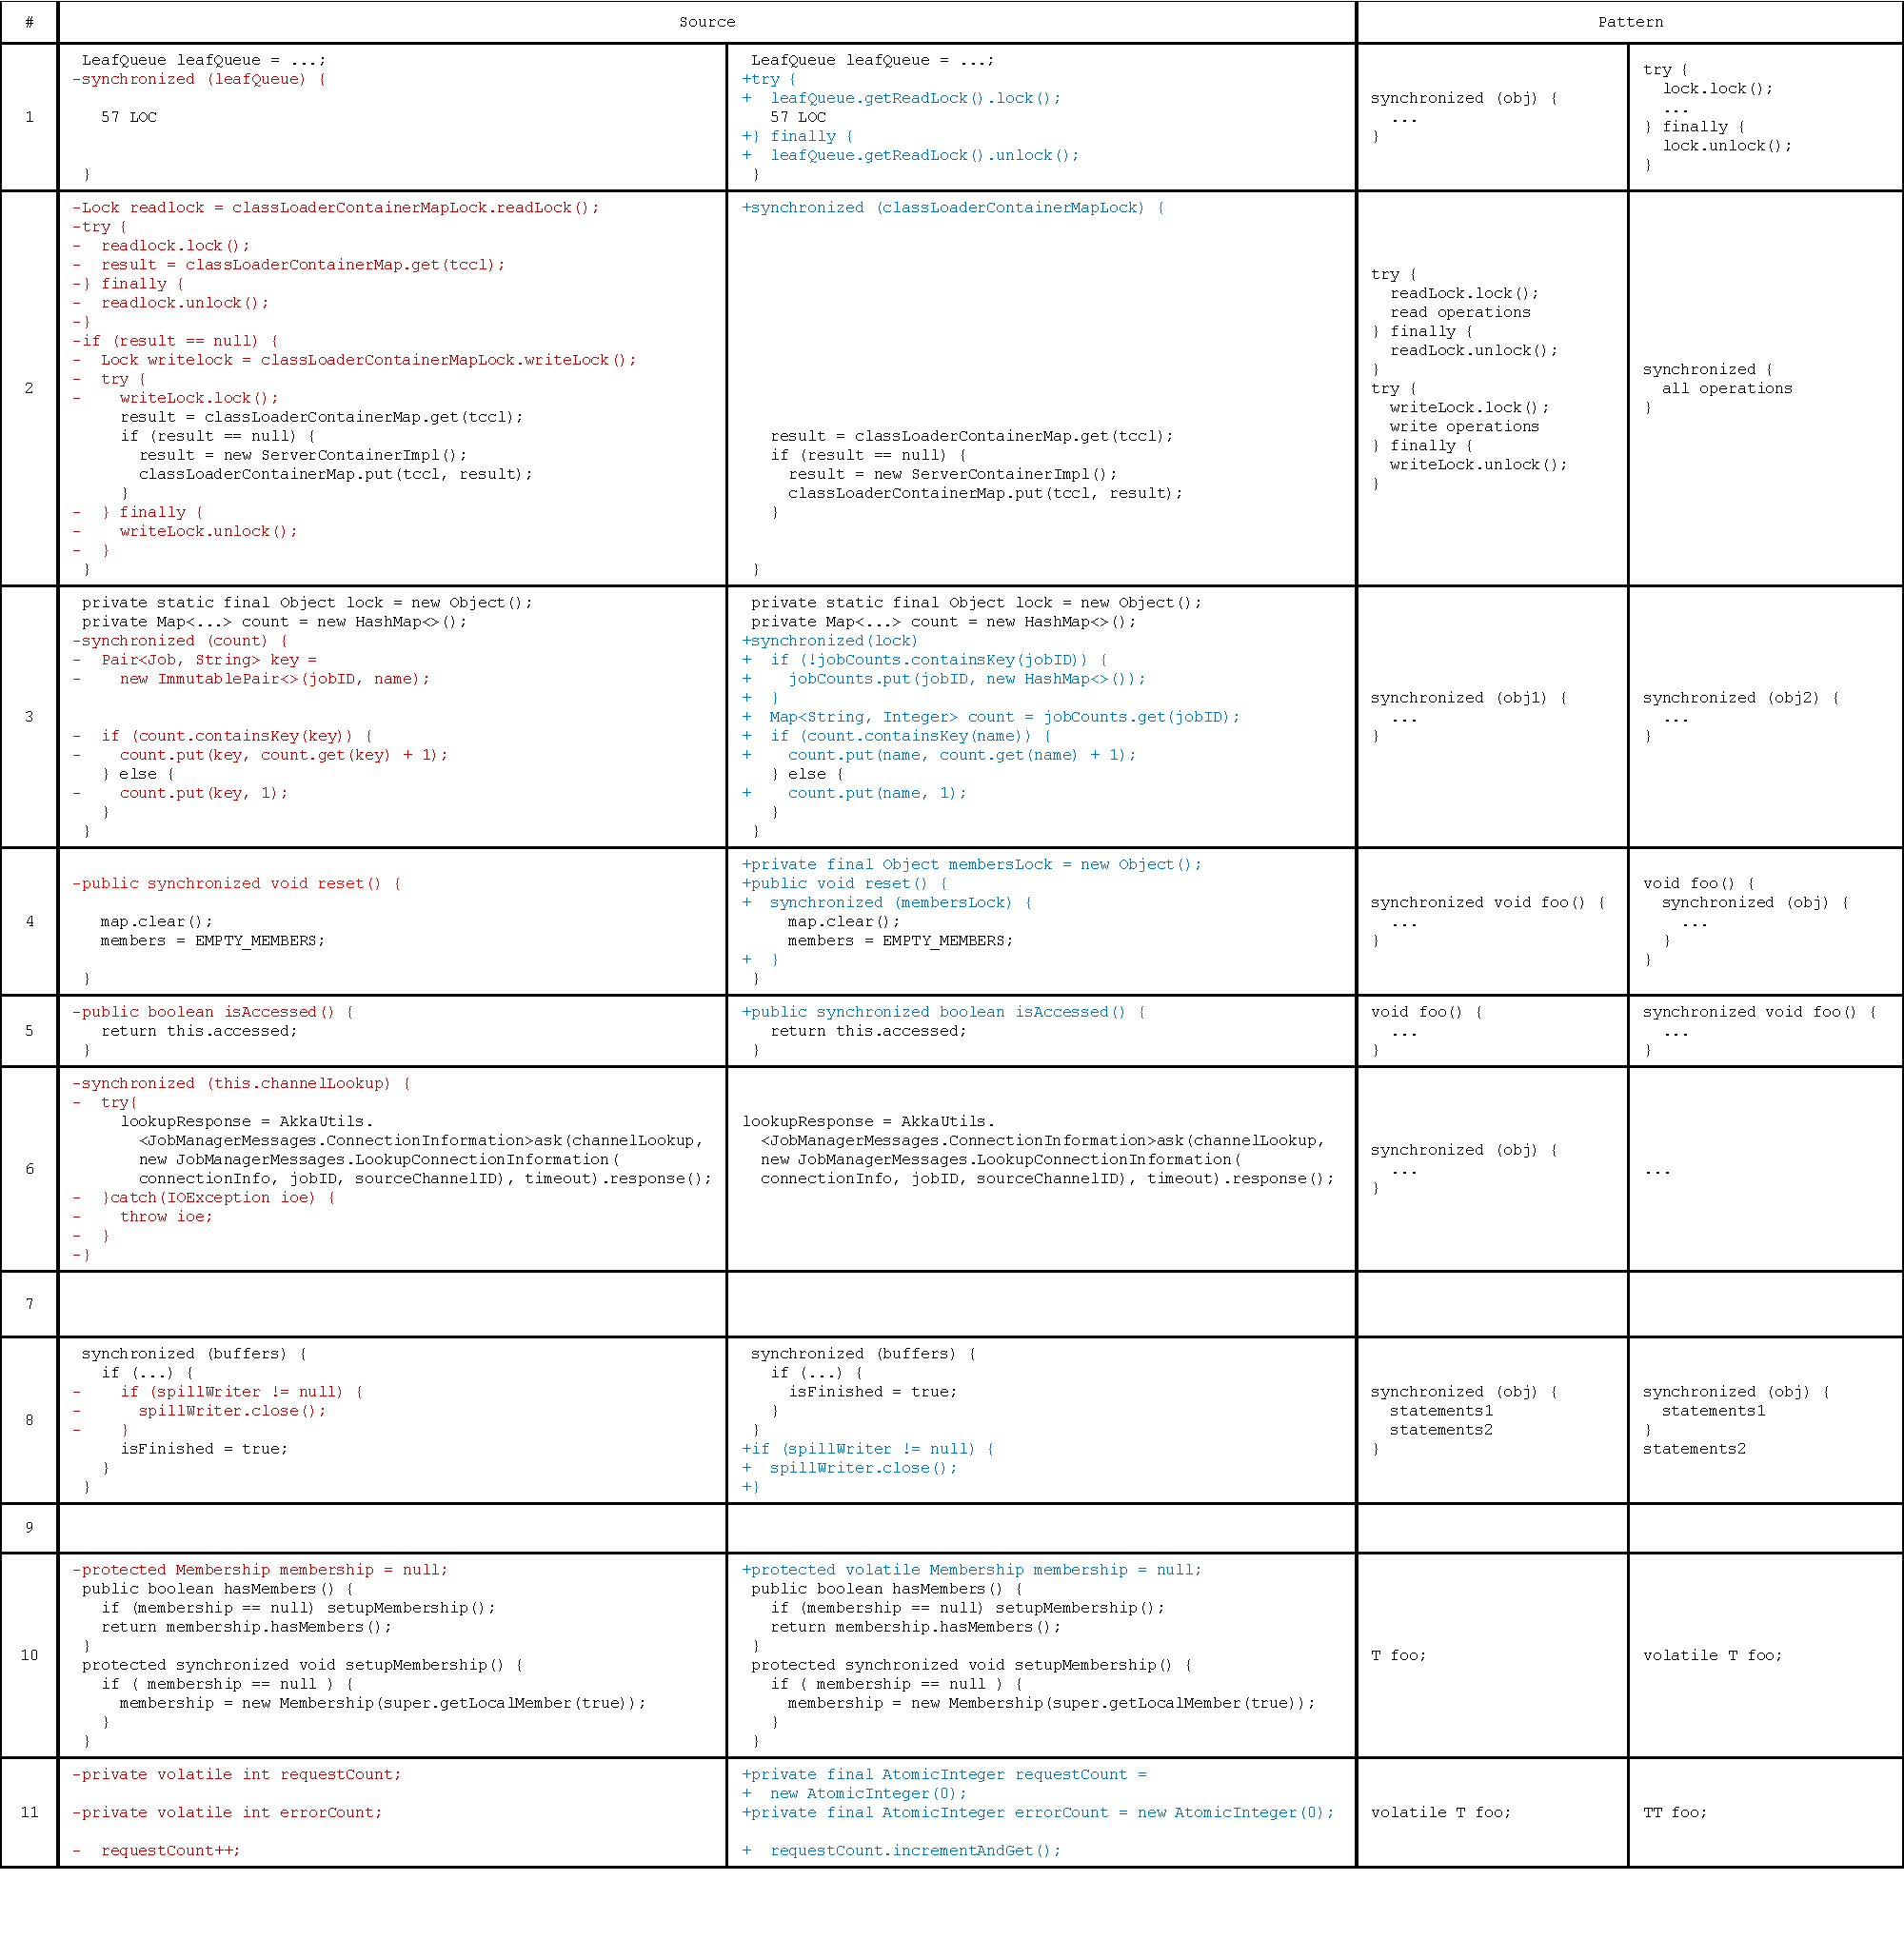
\includegraphics[width=1\textwidth]{patterns}	
	\label{table:patterns}

\end{table*}
\begin{table*}
	\centering
	\caption{Change patterns (Cont.)}\vspace*{-3ex}
	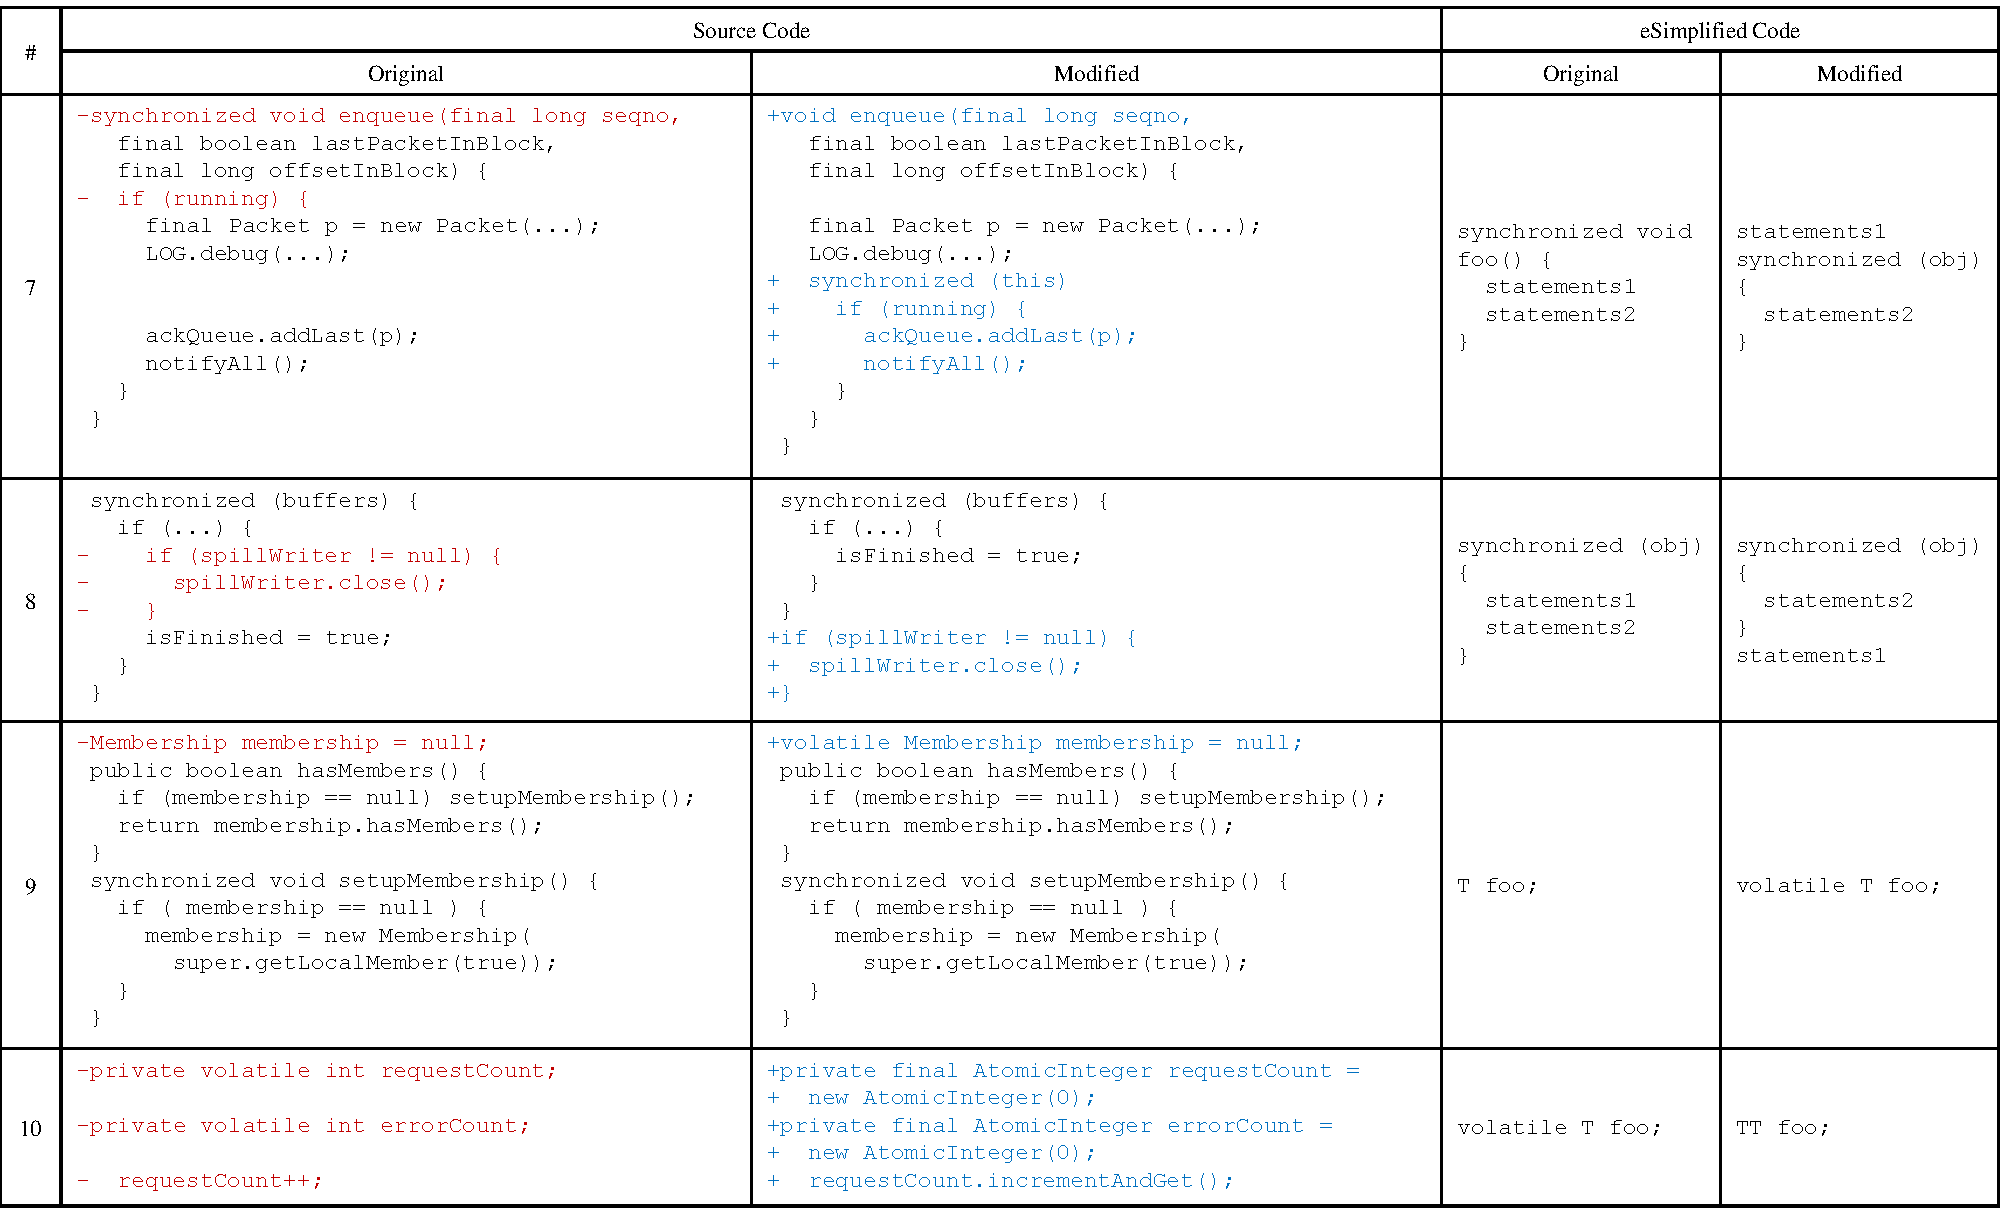
\includegraphics[width=1\textwidth]{patterns2}
	\label{table:patterns2}
\end{table*}
\noindent
\textbf{1. Changing lock types.} It is feasible to lock resources with different mechanisms. For example, Java has a keyword, \CodeIn{synchronized}. The keyword can lock a block of code lines. With the keyword, programmers do not have to acquire and release resources explicitly. Alternatively, programmers can explicitly lock resources with APIs (\emph{e.g.}, \CodeIn{ReentrantLock}). Explicit locks offer more features that the \CodeIn{synchronized} keyword does not. For example, with such APIs, programmers can determine the conditions for a lock. As another example, besides exclusive locks, programmers can use shared locks. When a thread is holding an exclusive lock, other threads have to wait until it is released. In the contrast, shared locks allow multiple threads to hold the lock with specific actions. For example, \CodeIn{ReadWriteLock} allows multiple read actions, but denies multiple write actions.%\zhong{Please explain what exclusive and shared locks are, and their benefits.}

%ReentrantLock, ReentrantReadWriteLock, StampedLock are all API level locks in Java. Although 'synchronized' keyword is convenient and straightforward, we need other locks when we have more requirements. ReentrantLock is a reentrant lock, which means a lock can be acquired repeatedly in the same thread. It is a exclusive lock with the similar behaviour as monitor lock but has more features such as fairness, condition and tryLock. ReadWriteLock is a pair of locks, which allows concurrent access to read operations when there is no write operation going on but exclusive access to write operations. StampedLock is a lock which provides three modes, namely writing, reading and optimistic reading. This lock is usually used in design of thread-safe classes.
%Programmers can change their lock types due to various considerations. For example, the \CodeIn{synchronized} keyword can fail to satisfy fairness (\zhong{What is fairness? Why does it matter?}), programmers have to change such implicit locks to explicit locks. \zhong{Add an example for each situation.}

We find that programmers can replace the \CodeIn{synchronized} keyword with parallel API classes. For example, the first item of Table~\ref{table:patterns} comes from YARN-5825\footnote{\url{https://issues.apache.org/jira/browse/YARN-5825} To save space, we remove the URLs of the other Apache issues. Their URLs can be built by replacing the above URL with their issue number.}. To improve the performance, programmers replace the \CodeIn{synchronized} with the \CodeIn{getReadLock} method. The method returns a shared lock, so multiple threads can read the query simultaneously.

%3e4b1ae6dc786b268505aa2e64067432519c2bcf
%\begin{figure*}
%	\centering
%	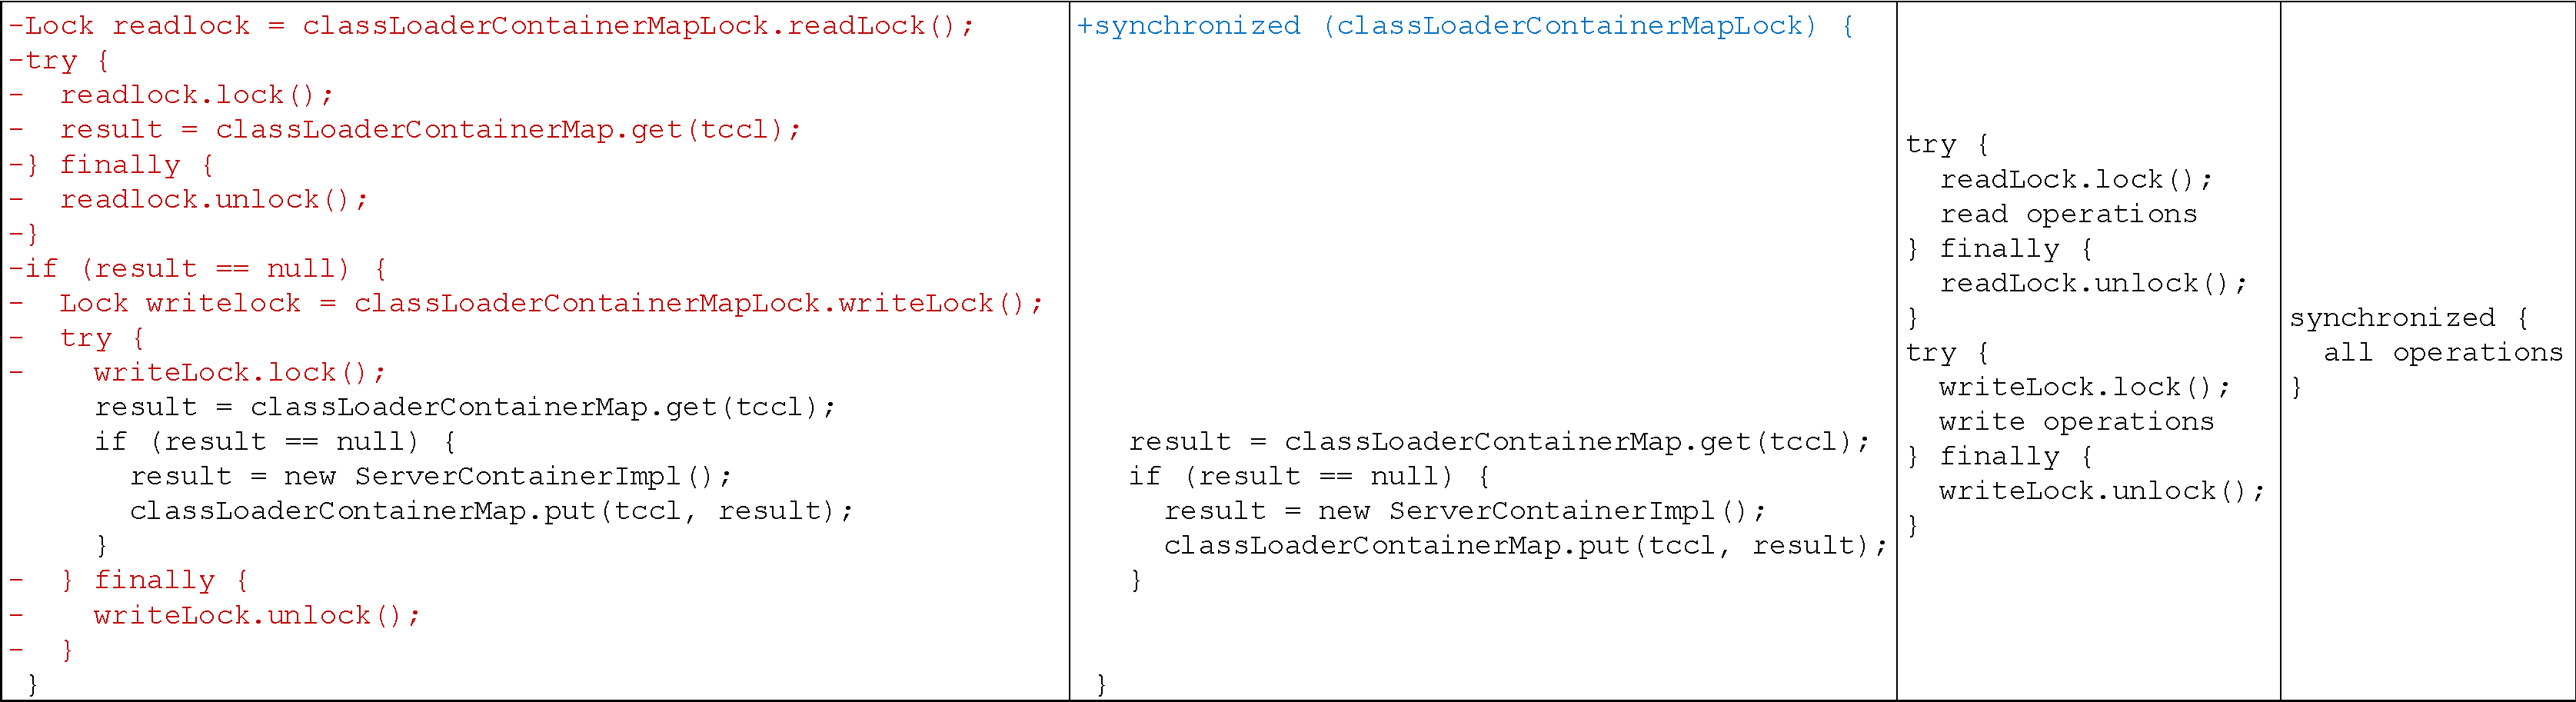
\includegraphics[scale=0.3]{locktype2}
%	\caption{Example 2}
%\zhong{It may be better, if you merge the example figures into a table like Table 1.}
%\end{figure*}

%\zhong{Please replace all texttt with CodeIn.}

%They also might switch to a reader-writer lock \cite{journals/cacm/CouroisHP71} from a normal lock to improve concurrency when there are plenty of concurrent read operations. Here are some examples. \zhong{add an example for this.}
Meanwhile, we find that programmers can replace parallel API classes with the \CodeIn{synchronized} keyword. For example, the second item of Table~\ref{table:patterns} comes from Tomcat\footnote{\url{https://svn.apache.org/viewvc?view=revision&revision=1414150}}. This commit is not reported, and we find it through our SVM classifier.% \zhong{List the commit message/log}.

%3e4b1ae6dc786b268505aa2e64067432519c2bcf
\begin{lstlisting}
A ReadWriteLock cannot be used to guard a WeakHashMap. The WeakHashMap may modify itself on get(), as it processes the reference queue of items removed by GC. Either a plain old lock / synchronization is needed, or some other solution.
\end{lstlisting}

As the above message explains, a developer complained that the \CodeIn{ReadWriteLock} method does not guard the \CodeIn{WeakHashMap} variable, since the \CodeIn{get()} method can modify the \CodeIn{WeakHashMap} variable, and the modification can bypass the lock. In this example, programmers fix the problem by replacing the methods with the \CodeIn{synchronized} keyword.%todo more detail

%When they find that they only need a simple exclusive lock, they switch to synchronized block. \zhong{add an example for this}
%\begin{figure}
%	\centering
%	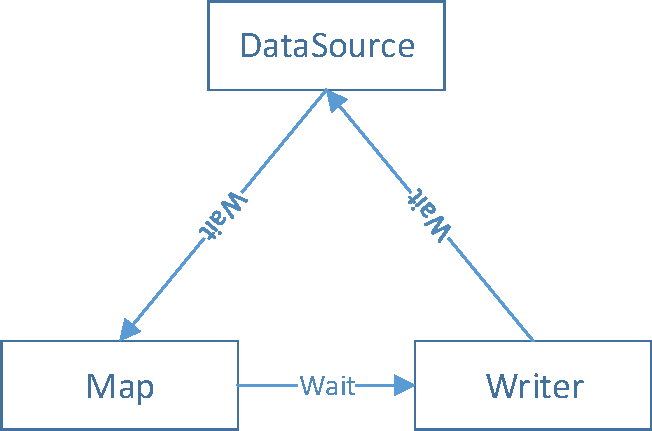
\includegraphics[height=1.7in]{deadlock}
%	\caption{Deadlock}
%	\label{figure:deadlock}
%%\zhong{Please add resource columns and add edges to denote resource manipulations.}
%\end{figure}

\noindent
\textbf{2. Changing locked variables.} A program needs to lock variables before it enters critical section bodies. During software maintenance, programmers can change locked variables, and we find that the main purpose is to repair bugs. For example, the third item of Table~\ref{table:patterns} comes from FLINK-1419. This bug complains that \CodeIn{DistributedCache} does not preserver files for subsequent operations. Based on its discussions, we understand that in the buggy file, programmers lock \CodeIn{count}, while they shall lock \CodeIn{lock}. To fully fix the bug, programmers also modified the critical sections and the \CodeIn{finally} clause.

As another example, when repairing bugs, programmers can add new locks. For example, the fourth item of Table~\ref{table:patterns} comes from Tomcat\footnote{\url{https://bz.apache.org/bugzilla/show\_bug.cgi?id=58386}}. It includes the following message:

\begin{lstlisting}
Reported by RV-Predict (a dynamic race detector) when running the test suite:
Data race on field org.apache.catalina.tribes.io.ObjectReader.accessed: {{{
Concurrent write in thread T93 (locks held: {...})
\end{lstlisting}

The data race indicates that the \CodeIn{isAccessed()} is not locked, so programmers add the \CodeIn{synchronized} keyword to allow locking on the method.


We find that programmers can also delete unnecessary locks. For example, the fifth item of Table~\ref{table:patterns} comes from Flink:

\begin{lstlisting}
...Remove synchronized blcok in getReceiverList of ChannelManager which effectively serialized the connection lookup calls of a single task manager.
\end{lstlisting}
%\zhong{show the URL of the commit}.
%\zhong{show what programmers say. Why it is unnecessary}.

As the above commit messages says, programmers removed synchronization from the \CodeIn{ChannelManager} class to improve the performance.


%\zhong{show the URL of the commit}.
%\zhong{show what programmers say. Why it is unnecessary}.




%\zhong{Why do you present the above stack trace.}

%\zhong{Instead of why a deadlock occurs, you shall explain why the modification in Table~\ref{table:patterns2} repaired the deadlock. If the modification alone is insufficient, add more details here.}
%As shown in Figure~\ref{figure:deadlock}, a deadlock can occur when three threads execute in a specific order. Here, we use $s1$ and $s2$ to denote two statements. An arrow from $s1$ to $s2$ means $s1$ cannot be returned before $s2$ has been returned. The \CodeIn{DataSource} (thread-1) is waiting to be notified by the \CodeIn{Writer} (thread-2) when holding lock A. The \CodeIn{Writer} (thread-2) is trying to acquire lock B. But lock B is held by the \CodeIn{Map} (thread-3). And the \CodeIn{Map} (thread-3) is trying to acquire lock A, which is held by the \CodeIn{DataSource} (thread-1). Here is a waiting chain. This is a kind of bug known as deadlock. The problem is that the \CodeIn{DataSource} (thread-1) does not need to hold lock A while waiting to be notified. So the developer removed the unnecessary synchronization.

%f0e627bb8c9daedb3b064027cac37ce4849bab64
In some other cases, we find that programmers can refine their locked resources to improve performance. For example, the seventh item of Table~\ref{table:patterns} comes from Tomcat\footnote{\url{https://bz.apache.org/bugzilla/show_bug.cgi?id=58382}}. The original code locks the instance of a class, but the modified code locks only the \CodeIn{membersLock} field.

\noindent
\textbf{3. Modifications inside critical section bodies.} A critical section is a code block that is executed, when a thread locks the corresponding resources. We notice that even modifications inside critical section bodies can repair concurrency bugs. For example, the sixth item of Table~\ref{table:patterns2} comes from FLINK-2384. It reports a deadlock that produces the following stack trace:

\begin{lstlisting}
"CHAIN DataSource (at createInput(ExecutionEnvironment.java:502) (org.apache.flink.api.java.hadoop.mapreduce.HadoopInputFormat)) -> FlatMap (FlatMap at readFlinkTuplesFromThriftParquet(ParquetThriftEntitons.java:96)) (7/8)" daemon prio=10 tid=0x00007f934005b000 nid=0x73c4 in Object.wait() [0x00007f93c16ac000]
java.lang.Thread.State: TIMED_WAITING (on object monitor)

"IOManager writer thread #1" daemon prio=10 tid=0x00007f93d8b7b000 nid=0x73a8 waiting for monitor entry [0x00007f93c2fc5000]
java.lang.Thread.State: BLOCKED (on object monitor)

"Map (Projection [0, 1, 2, 3, 4]) (7/8)" daemon prio=10 tid=0x00007f92b0434800 nid=0x74a3 waiting for monitor entry [0x00007f93a32f1000]
java.lang.Thread.State: BLOCKED (on object monitor)
\end{lstlisting}

The stack trace indicates that the \CodeIn{spillWriter.close()} method has an implicit lock. As programmers typically do not known such locks inside APIs, the lock leads to the deadlock. Indeed, we find that a recent benchmark~\cite{lin2015ase} includes a similar concurrency bug, and Lin \emph{et al.}~\cite{lin2016lockpeeker} proposed an approach that detects such implicit locks inside APIs. In this example, programmers move the \CodeIn{spillWriter.close()} method outside the critical section body to resolve the deadlock.


%<<<<<<< HEAD
%f0e627bb8c9daedb3b064027cac37ce4849bab64
%In some other cases, we find that programmers can refine their locked resources to improve performance. For example, the seventh item of Table~\ref{table:patterns} comes from Tomcat\footnote{\url{https://bz.apache.org/bugzilla/show_bug.cgi?id=58382}}. The original code locks the instance of a class, but the modified code locks only the \CodeIn{membersLock} field.

%\noindent
%\textbf{3. Modifications on critical section bodies.} A critical section is a code block that is executed, when a thread locked the corresponding resources. The modifications on critical section bodies indicate new functionalities or refactoring. For example, the eighth item of Table~\ref{table:patterns2} comes from HDFS-4200. To reduce the size of a critical section body, programmers refactor the body into several methods. Indeed, this issue involves modifications that are related to even more change patterns (\emph{e.g.}, adding locked variables).
%=======
Besides the above example, the majority of modifications on critical section bodies indicates new functionalities or refactoring. For example, the eighth item of Table~\ref{table:patterns2} comes from HDFS-4200. To reduce the size of a critical section body, programmers refactor the body into several methods. Indeed, this issue involves modifications that are related to even more change patterns (\emph{e.g.}, adding locked variables).
%>>>>>>> 9e8b767a2cf136027178c18c50d9c5eea616e630

%c93d9eaf363a535dff25cc4e7db400d879e73bb1
%Add option to use single actor system for local execution. Use local connection manager if a single task manager is used for local execution. Remove synchronized blcok in getReceiverList of ChannelManager which effectively serialized the connection lookup calls of a single task manager.
%\zhong{Why do you list the following commits? If you cannot list the following commit in Table~\ref{table:patterns2}, split it into the original code and fixed code. Explain them separatively.}

%Modifications on statements change statements of critical sections.

%efca79cfb7b496b4bec70561cc94af069c644ef2
%[FLINK-2384] [runtime] Move blocking I/O call outside of synchronized block
%Problem: Waiting on asynchronous write requests with the partition lock can
%result in a deadlock, because all other operations on the same partition are
%blocked. It is possible that the I/O writer itself needs to access the
%partition, in which cases the whole program blocks.
%Solution: Move the wait outside the synchronized block. This was not necessary
%before, because no operation assumes the spilling to be finished when the
%finish call has returned.




%Modifications on locked resources change the criteria of entering critical sections.  \zhong{Please check whether the samples explain the corresponding situations.}



%Example 9.



\noindent
\textbf{4. Changing the \CodeIn{volatile} keyword.} In Java, the \CodeIn{volatile} keyword denotes a variable that is saved in the main memory. For a \CodeIn{volatile} variable, a thread reads its latest value from the main memory, instead of the obsolete  value in the cache. Although it can improve the overall performance, races can occur, when multiple threads read and write \CodeIn{volatile} variables simultaneously.

%8313fa0f1ca277e9633a78f461804abc3c5515b8
%Fix https://bz.apache.org/bugzilla/show_bug.cgi?id=58392
%Double-checked locking needs to use volatile to be thread-safe
We find that programmers can add the \CodeIn{volatile} keyword to improve performance. For example, the ninth item of Table~\ref{table:patterns2} comes from Tomcat\footnote{\url{https://bz.apache.org/bugzilla/show_bug.cgi?id=58392}}. It reports a data race, and the bug was repaired by adding the \CodeIn{volatile} keyword.

%560cd00890b3f6af2aca0c3a9d51a45f880692dd
%Fix a FindBugs warning (increment of volatile not atomic)

%\zhong{Please explain why you need two samples for this situation.}
Besides adding the keyword, we find that programmers have to remove the \CodeIn{volatile} keyword, since they do not fully understand its meanings. For example, in tenth item of Table~\ref{table:patterns2} comes from Tomcat\footnote{\url{https://svn.apache.org/viewvc?view=revision&revision=1360946}}. In this bug, programmers auto-increment a \CodeIn{volatile} variable, but such an action is not atomic. As a result, FindBugs reports it as a bug, and programmers have to remove the keyword.

\noindent
\textbf{5. Replacing self-written code with Parallel APIs.} Programmers can implement concurrent code by themselves, but later they realize that it is easier to call APIs that already implement their functionalities. For example, a previous version of Hadoop has the following code:% \zhong{Replace the below commit with the buggy code.}

%\begin{lstlisting}
%commit a258263ecfa1d9efe03761f5e3b73e8e6ddb4a43
%HDFS-4029. GenerationStamp should use an AtomicLong. Contributed by Eli Collins
%
%-  private volatile long genstamp;
%+  private AtomicLong genstamp = new AtomicLong();
%...
%-  public synchronized long nextStamp() {
%-    this.genstamp++;
%-    return this.genstamp;
%+  public long nextStamp() {
%+    return genstamp.incrementAndGet();
%   }
%\end{lstlisting}

\begin{lstlisting}
private volatile long genstamp;
public synchronized long nextStamp() {
  this.genstamp++;
  return this.genstamp;
}
\end{lstlisting}

Later, a programmer realized that it is better to replace the above code with the \CodeIn{AtomicLong} class. He reported the issue (HDFS-4029), and set its priority as major. Here, \CodeIn{AtomicLong} is a thread-safe version of type long. It allows updating a \CodeIn{Long} value without explicit synchronization and it is fast.

%It not only offers a simple interface, but also has a different implementation than the example code above. It uses \CodeIn{Unsafe} class, which provides unsafe operations as its name represents. This class allows low-level programming in Java, which is considered unsafe but can save running time without the check to guarantee safety. It might be promoted to be public API in Java 9. The fixed code is as follow:

%\zhong{Replace the below commit with the fixed code.}

\begin{lstlisting}
private volatile long genstamp;
public long nextStamp() {
  return genstamp.incrementAndGet();
}
\end{lstlisting}

Besides replacing directly, programmers can replace their code with parallel APIs that implement similar functions. For example, the below code comes from LUCENE-2779:

\begin{lstlisting}
  protected HashMap<String,RAMFile> fileMap = new HashMap<String,RAMFile>();
  ...
  public final boolean fileExists(String name) {
    ensureOpen();
    RAMFile file;
    synchronized (this) {
      file = fileMap.get(name);
    }
    return file != null;
 }
\end{lstlisting}

Instead of handling synchronization by themselves, programmers replaced the above code with a parallel API:

\begin{lstlisting}
 protected Map<String,RAMFile> fileMap = new ConcurrentHashMap<String,RAMFile>();
 ...
 public final boolean fileExists(String name) {
    ensureOpen();
    return fileMap.containsKey(name);
 }
\end{lstlisting}

%\textbf{Other class replace}
%
%\textbf{Thread resource management}
%
%When we do concurrent programming, we need to pay attention to resource management such as threads, locks.
%
%Thread management is to deal with the management of thread-related resources.
%
%\textbf{Thread sleep wait notify}
%
%It is a another way of synchronization which is less common than locking.
%
%\textbf{Final in multiple threads}

In summary, in our study, we identify five types of change patterns in total. First, we find that programmers can modify parallel keywords and locked variables, and such modifications are mainly for repairing bugs and improving performance. Second, we notice modifications on critical section bodies, and such modifications often indicate new functions. Finally, we notice that self-written code is replaced with corresponding parallel APIs. In most cases, we find that maintaining concurrent code is not a one-direction migration. For example, there are several different ways to implement a lock. Programmers shall carefully analyze their programming contexts to determine which is their best choice. As shown in our examples, during software maintenance, programmers can migrate to any types according to their need.

\subsection{RQ2. The usefulness of our change patterns.}
\label{sec:result:sample}

%\zhong{Try to add an example for each change pattern.}
%\zhong{How many pull requests did you submit?}

In total, we made three pull requests. We made the first pull request on Schmince-2\footnote{\url{https://github.com/derekmu/Schmince-2}}. This is a game, where players control space tourists for adventure. It has the following code:

\begin{lstlisting}
public class DRandom {
  private static ThreadLocal<Random> random = new ThreadLocal<Random>() {
    protected Random initialValue() {
      return new Random();
    }
  };
  public static Random get() {
    return random.get();
  }
}
\end{lstlisting}

The above code implements a class that generates random values for multiple threads. We find that J2SE provides the \CodeIn{ThreadLocalRandom} class\footnote{\url{https://docs.oracle.com/javase/8/docs/api/java/util/concurrent/ThreadLocalRandom.html}} that implements the identical function. According to our fifth change pattern, we made a pull request to replace the above code with the corresponding API\footnote{\url{https://github.com/derekmu/Schmince-2/pull/1}}, and the modified code is as follow:

\begin{lstlisting}
public class DRandom {
  public static Random get() {
    ThreadLocalRandom.current();
  }
}
\end{lstlisting}
This pull request is already confirmed by programmers of the project.
%\begin{lstlisting}
%+import java.util.concurrent.ThreadLocalRandom;
%public class DRandom {
%-    private static ThreadLocal<Random> random = new ThreadLocal<Random>() {
%-        protected Random initialValue() {
%-            return new Random();
%-        }
%-    };
%public static Random get() {
%-        return random.get();
%+        ThreadLocalRandom.current();
%}
%}
%\end{lstlisting}

%This example shows a change from ThreadLocal$<$Random$>$ to ThreadLocalRandom from JDK7. It is from a Schmince-2, a game on Google Play. We make the change and our pull request\footnote{\url{https://github.com/derekmu/Schmince-2/pull/1}} has been accept. ThreadLocalRandom should be used when available in place of ThreadLocal$<$Random$>$. For JDK7 the difference is minimal, but JDK8 starts including optimizations for ThreadLocalRandom. The ThreadLocal class provides thread-local variables. The ThreadLocalRandom class is a random number generator isolated to the current thread.
\begin{figure*}
	\centering
	\subfigure[Ascending-high]{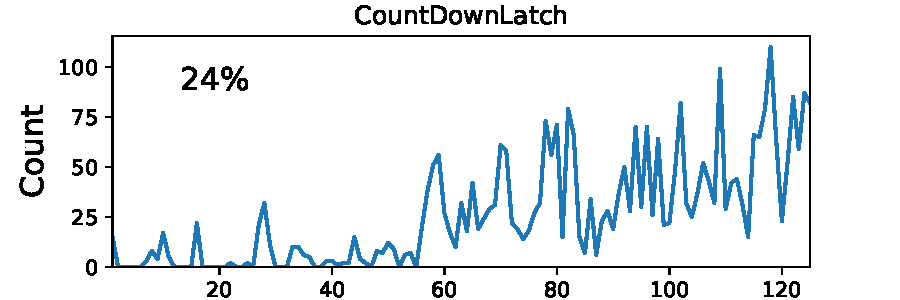
\includegraphics[width=2.3in]{CountDownLatch}}
	\subfigure[Descending-high]{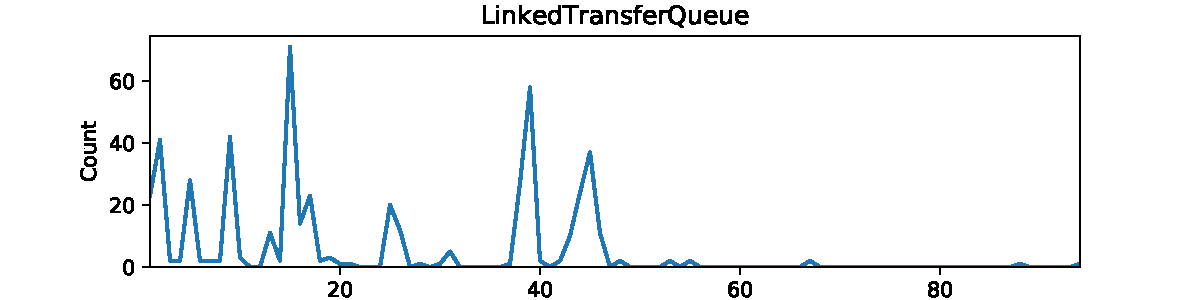
\includegraphics[width=2.3in]{LinkedTransferQueue}}
	\subfigure[Hybrid-high]{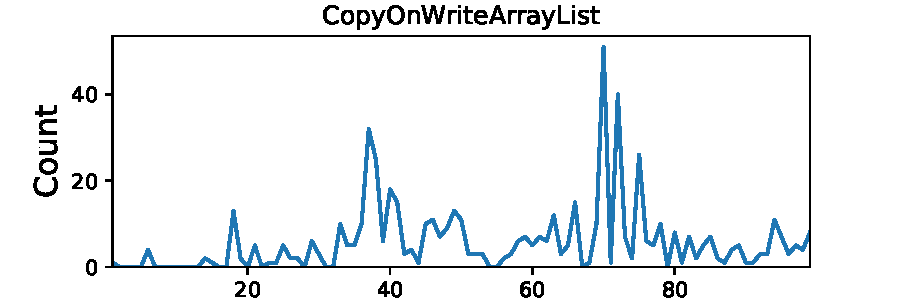
\includegraphics[width=2.3in]{CopyOnWriteArrayList}}
	
	\subfigure[Ascending-medium]{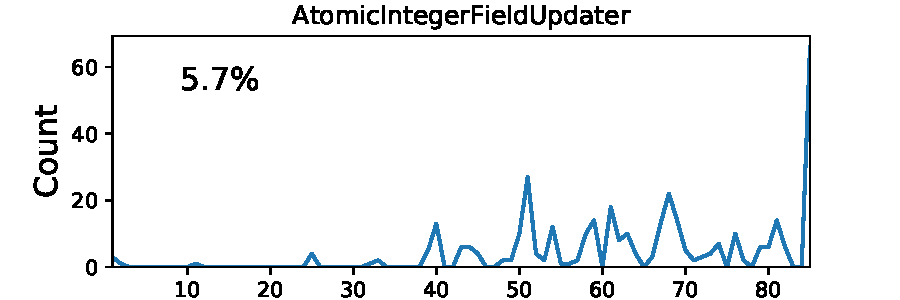
\includegraphics[width=2.3in]{AtomicIntegerFieldUpdater}}
	\subfigure[Descending-medium]{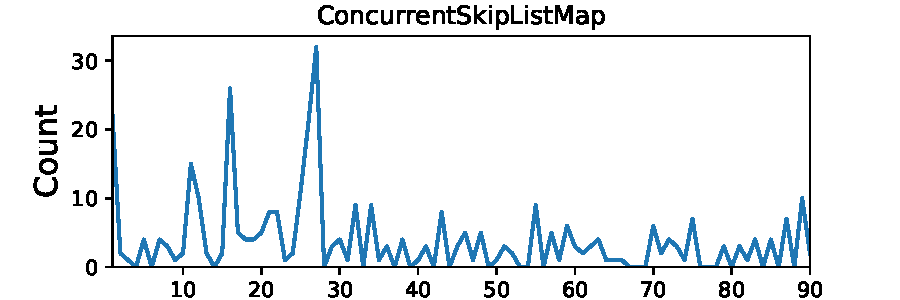
\includegraphics[width=2.3in]{ConcurrentSkipListMap}}
	\subfigure[Hybrid-medium]{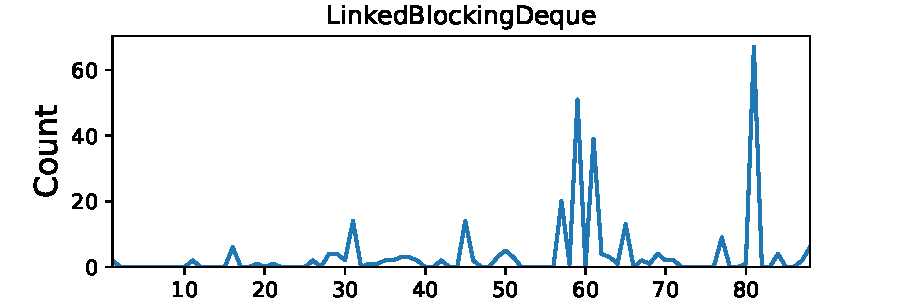
\includegraphics[width=2.3in]{LinkedBlockingDeque}}
	
	\subfigure[Ascending-low]{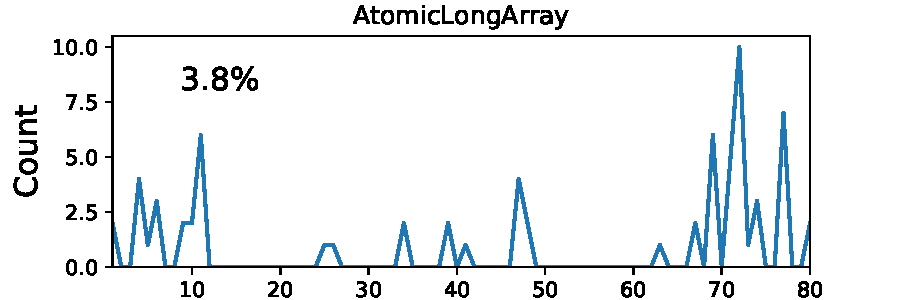
\includegraphics[width=2.3in]{AtomicLongArray}}
	\subfigure[Descending-low]{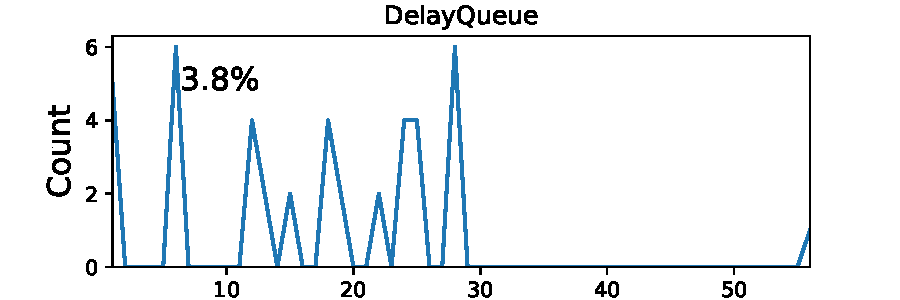
\includegraphics[width=2.3in]{DelayQueue}}
	\subfigure[Hybrid-low]{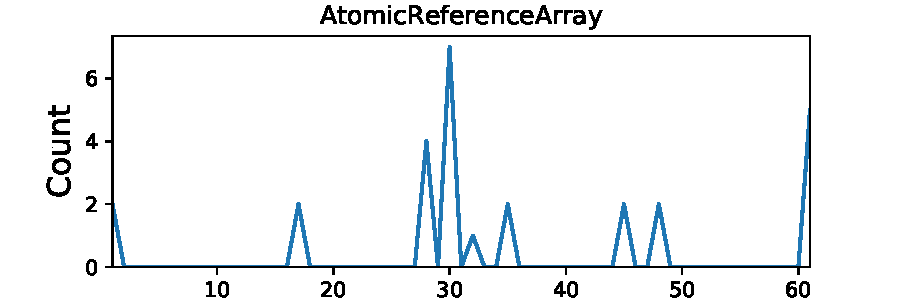
\includegraphics[width=2.3in]{AtomicReferenceArray}}
	
%	\subfigure[Descending]{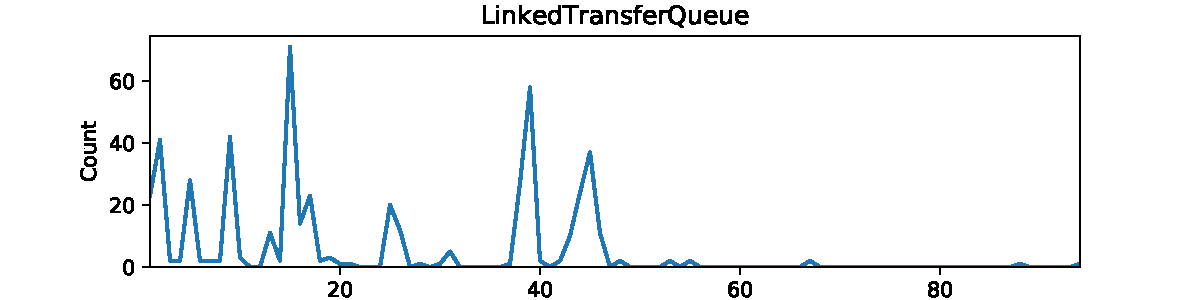
\includegraphics[width=2.3in]{LinkedTransferQueue}}
%	\subfigure[Hybrid]{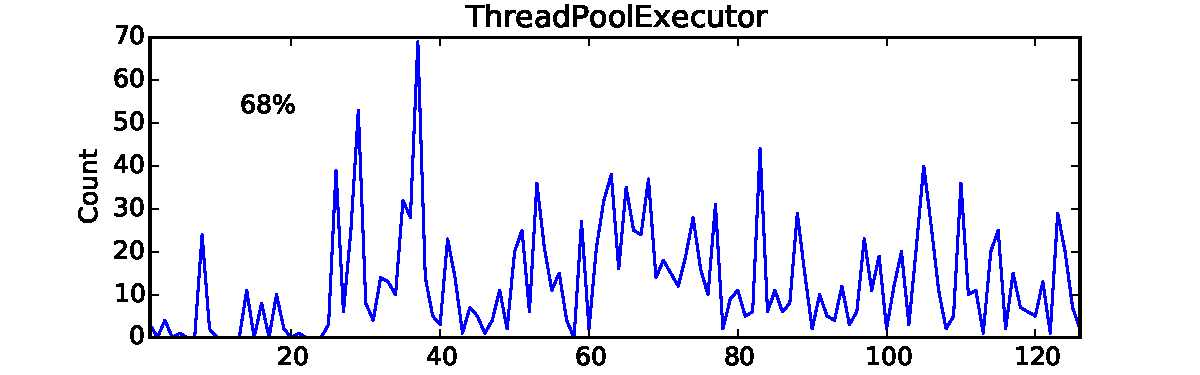
\includegraphics[width=2.3in]{ThreadPoolExecutor}}
%	\subfigure[High]{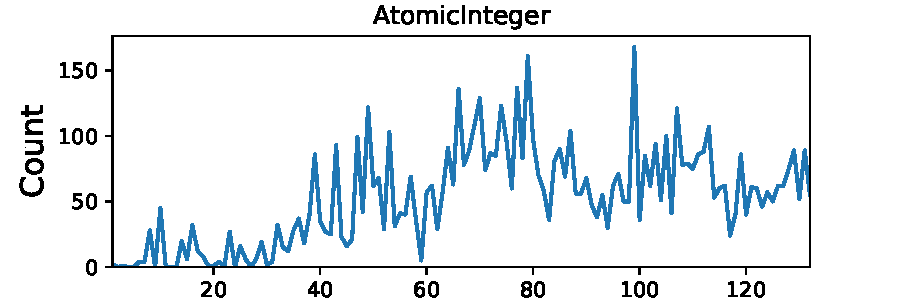
\includegraphics[width=2.3in]{AtomicInteger}}
%	\subfigure[Medium]{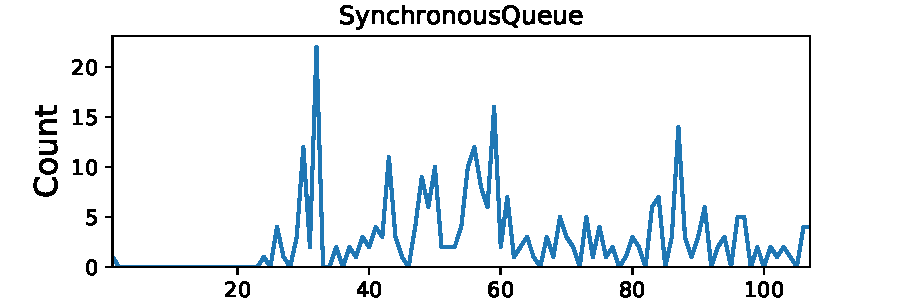
\includegraphics[width=2.3in]{SynchronousQueue}}
%	\subfigure[Low]{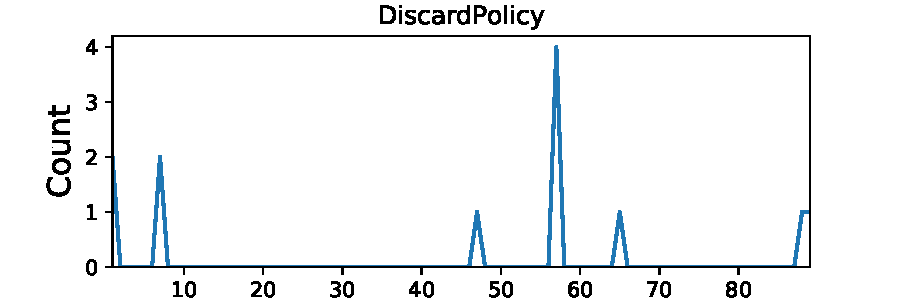
\includegraphics[width=2.3in]{DiscardPolicy}}
	\caption{Typical trends and their percents}
	\label{figure:trend}\vspace*{-3ex}
%\zhong{The labels shall be like ascending-high, ascending-medium, ascending-low, and etc. There shall be nine graphs in total. The percents of the nine graphs shall add up to 100\%.}
\end{figure*}
We made the second pull request on UnifiedEmail\footnote{\url{https://github.com/HexagonRom/android_packages_apps_UnifiedEmail}}. It is an Android email client. It has the following code:

\begin{lstlisting}
private static NotificationMap sActiveNotificationMap = null;
private static synchronized NotificationMap getNotificationMap(Context context) {
  if (sActiveNotificationMap == null) {
    sActiveNotificationMap = new NotificationMap();
    sActiveNotificationMap.loadNotificationMap(context);
  }
  return sActiveNotificationMap;
}
\end{lstlisting}

If the \CodeIn{sActiveNotificationMap} field is \CodeIn{null}, the above method creates a new map and assigns the new map to the field. To allow multiple threads to call the methods, programmers add the \CodeIn{synchronized} keyword to the method. We believe that when \CodeIn{sActiveNotificationMap} is not \CodeIn{null}, the lock is unnecessary, since it does not change the field. According to our second change pattern, we made the following modification to synchronize only the lines that modify the field:

\begin{lstlisting}
private static volatile NotificationMap sActiveNotificationMap = null;
private static NotificationMap getNotificationMap(Context context) {
  if (sActiveNotificationMap == null) {
    synchronized (NotificationUtils.class) {
      if (sActiveNotificationMap == null) {
        sActiveNotificationMap = new NotificationMap();
        sActiveNotificationMap.loadNotificationMap(context);
      }
    }
  }
  return sActiveNotificationMap;
}
\end{lstlisting}

The above pull request is still pending.
\begin{table}
	\centering
	\caption{Top 10 Active Classes}\vspace*{-2ex}
	\label{table:topapi}
	\begin{tabular}{|c|c|}\hline
		Class&Occurrence\\\hline
		AtomicInteger&6,891\\
		AtomicBoolean&4,180\\
		ConcurrentHashMap&3,976\\
		AtomicLong&3,926\\
		CountDownLatch&3,211\\
		AtomicReference&2,254\\
		Executors&2,026\\
		ThreadPoolExecutor&1,617\\
		LinkedBlockingQueue&1,553\\
		ConcurrentLinkedQueue&1,435\\\hline
	\end{tabular}\vspace*{-3ex}
\end{table}

We made the third pull request on Spider4java\footnote{\url{https://github.com/lichangshu/spider4java}}. It is a Java web crawler. It has the following code:


\begin{lstlisting}
public class Counter {
  protected int count;
  public Counter() {
    count = 0;
  }
  public synchronized void increment() {
    count = count + 1;
  }
  public synchronized int getValue() {
    return count;
  }
}
\end{lstlisting}

The above class implements a counter for multiple threads. As J2SE provides the identical API, \CodeIn{AtomicInteger}\footnote{\url{https://docs.oracle.com/javase/8/docs/api/java/util/concurrent/atomic/AtomicInteger.html}}, we modify it as follow:

\begin{lstlisting}
public class Counter {
  protected AtomicInteger count;
  public Counter() {
    count = new AtomicInteger();
  }
  public void increment() {
    count.getAndIncrement();
  }
  public int getValue() {
    return count.get();
  }
}
\end{lstlisting}
\begin{figure*}
	\centering
	\subfigure[Cassandra]{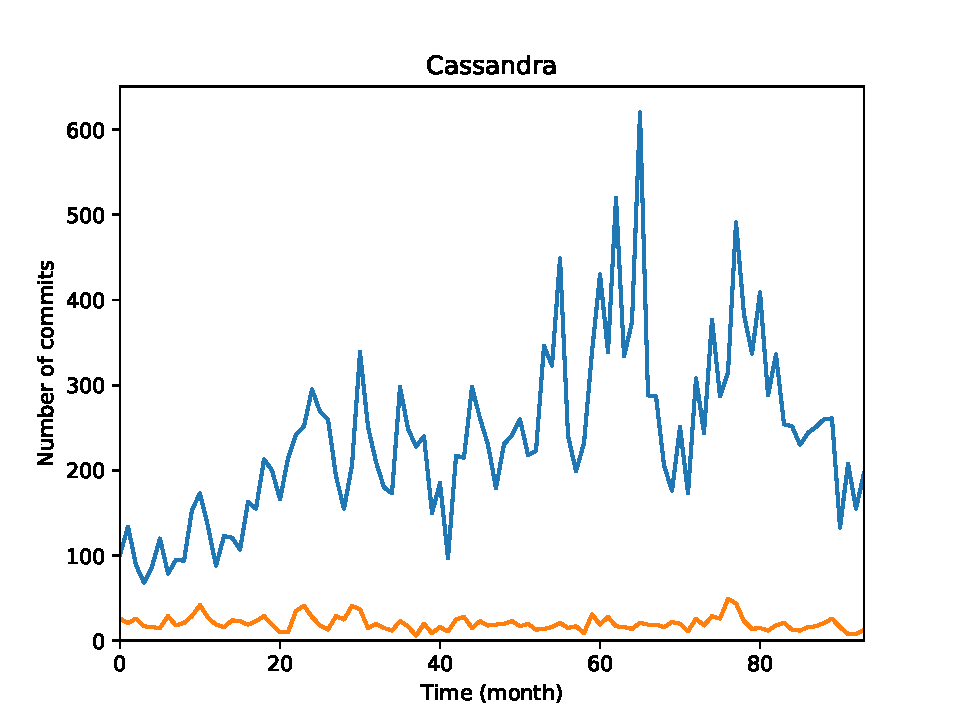
\includegraphics[height=1.4in]{cassandra}}
	\subfigure[Flink]{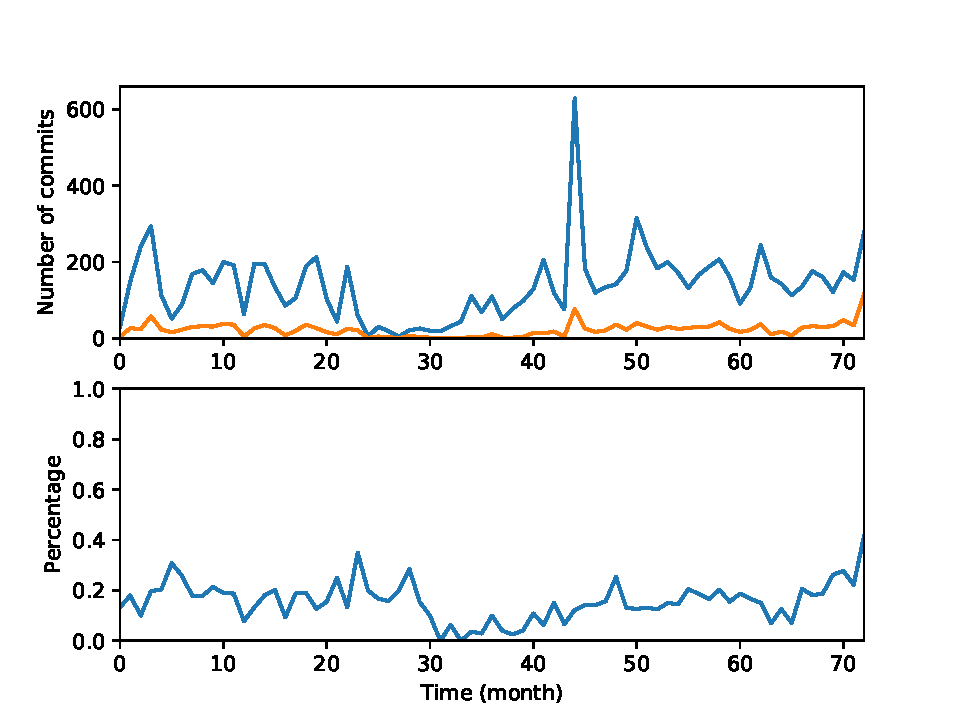
\includegraphics[height=1.4in]{flink}}
	\subfigure[Hadoop]{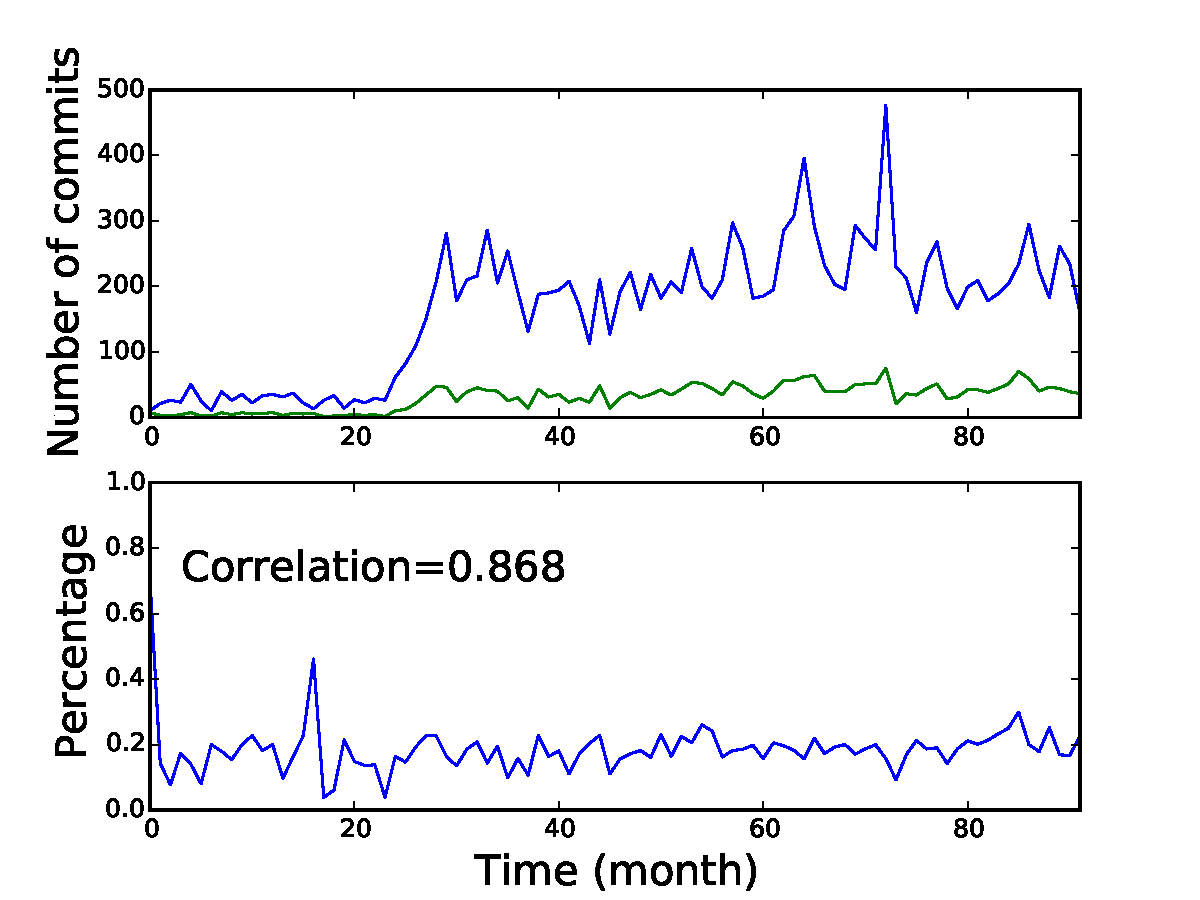
\includegraphics[height=1.4in]{hadoop}}
	\subfigure[Lucene-Solr]{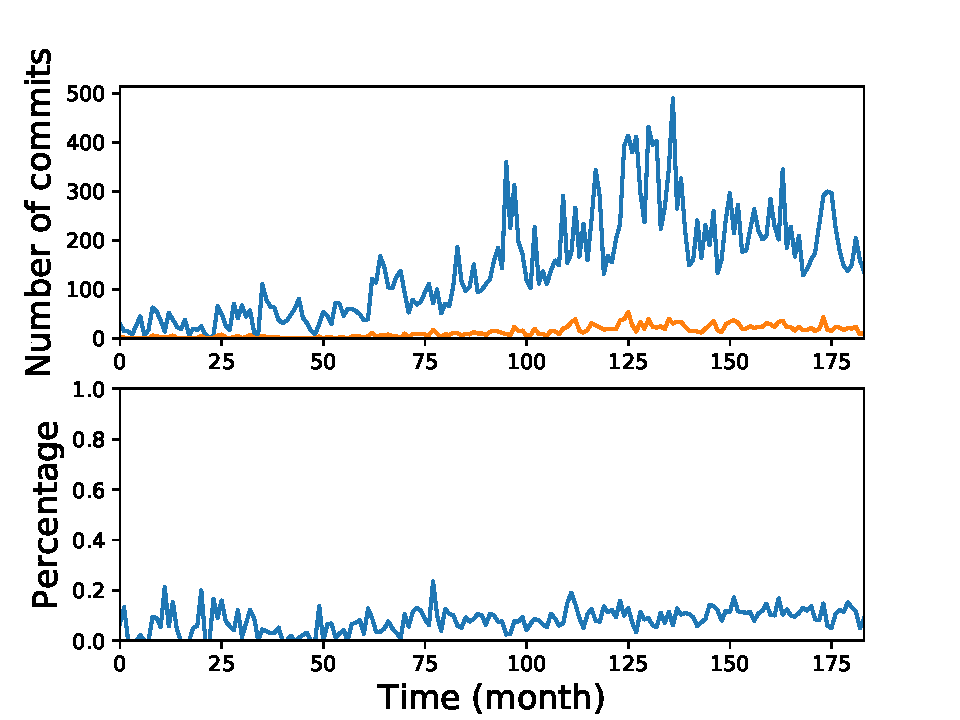
\includegraphics[height=1.4in]{lucene-solr}}
	%\subfigure[Mahout]{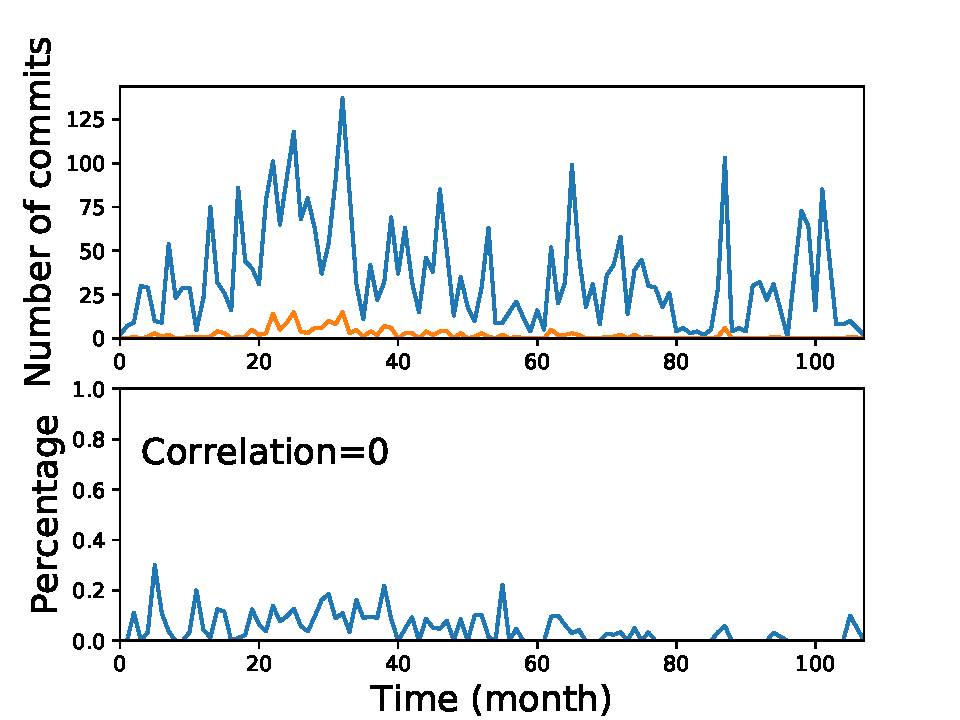
\includegraphics[height=1.2in]{mahout}}
	\subfigure[Netty]{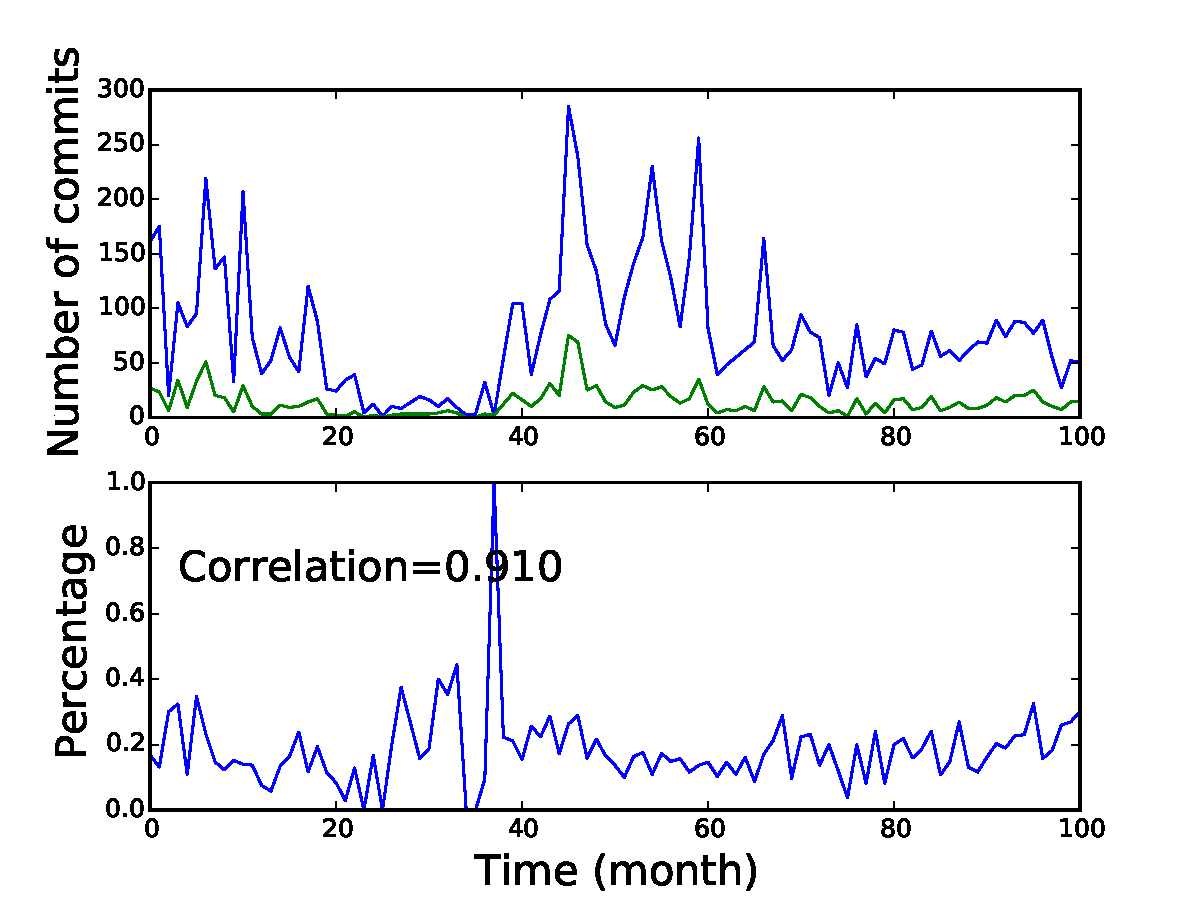
\includegraphics[height=1.4in]{netty}}
	\subfigure[Tomcat]{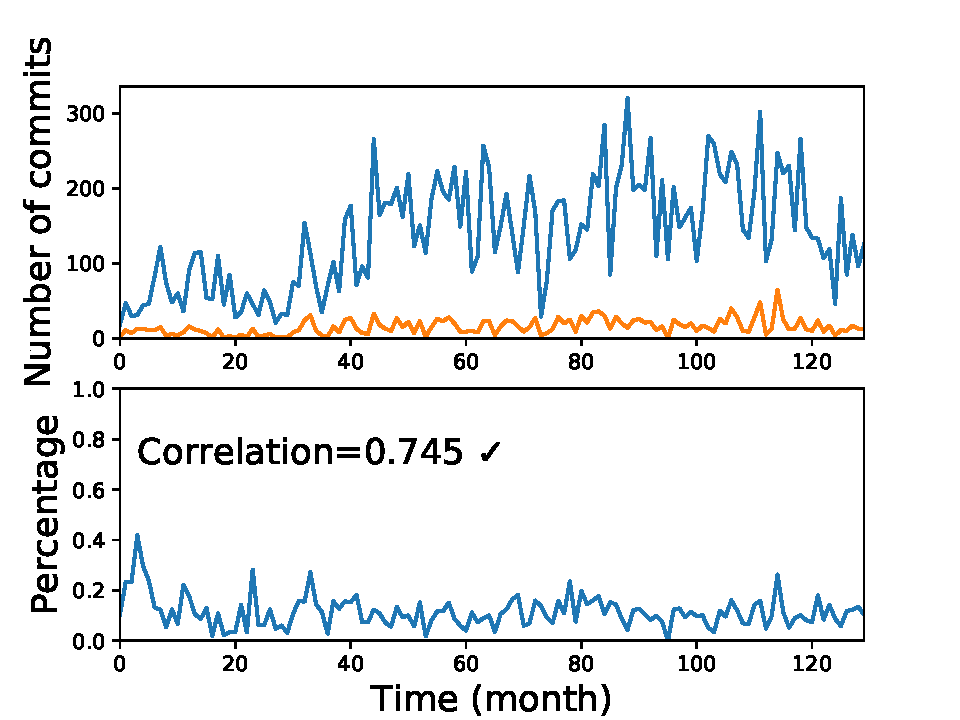
\includegraphics[height=1.4in]{tomcat}}
	\caption{Number of concurrency-related commits compared to all commits}%\vspace*{-3ex}
	\label{fig:confidence}\vspace*{-3ex}
\end{figure*}

However, their programmers denied the pull request. Although our pull request works, it is more neat to systematically replace the above \CodeIn{Counter} class with the \CodeIn{AtomicInteger} class. Their programmers may deny our pull request, simply because the wrapper style looks ugly.

In summary, our results show that our change patterns are repetitive in future maintenance, and programmers confirmed that our change patterns are useful. However, our results also reveal that it needs much programming experience to fully unleash the potential of our change patterns. We further discuss this issue in Section~\ref{sec:discuss}.

\subsection{RQ3. What are the change trends of using parallel APIs}
\label{sec:result:trend}


%\begin{figure}
%	\centering
%	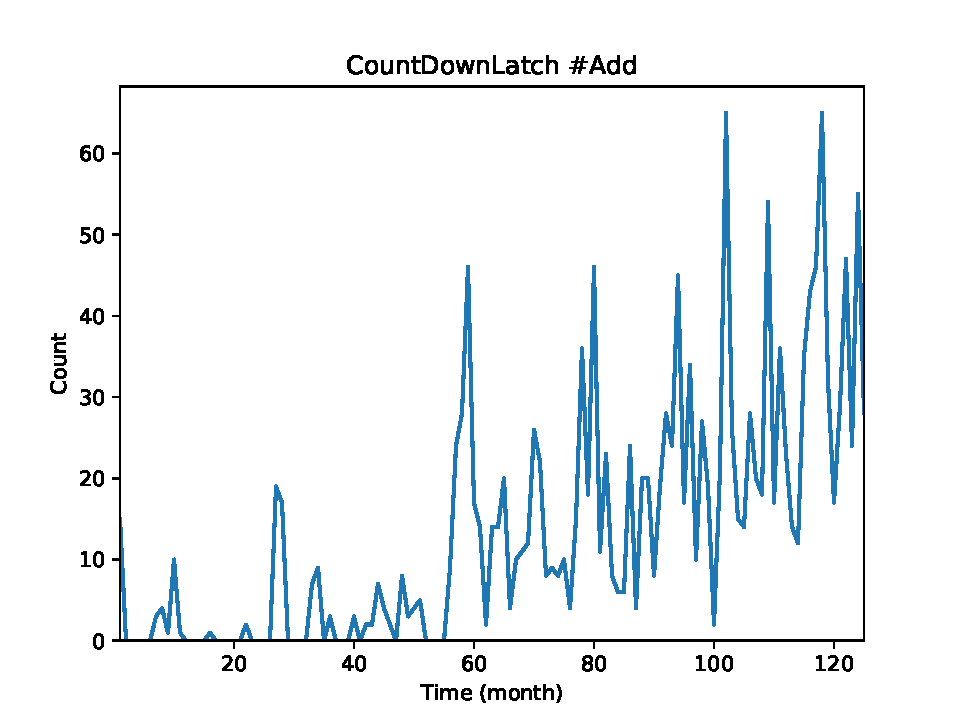
\includegraphics[height=1.5in]{CountDownLatchAdd}
%	\caption{Addition of CountDownLatch}
%\end{figure}
%
%\begin{figure}
%	\centering
%	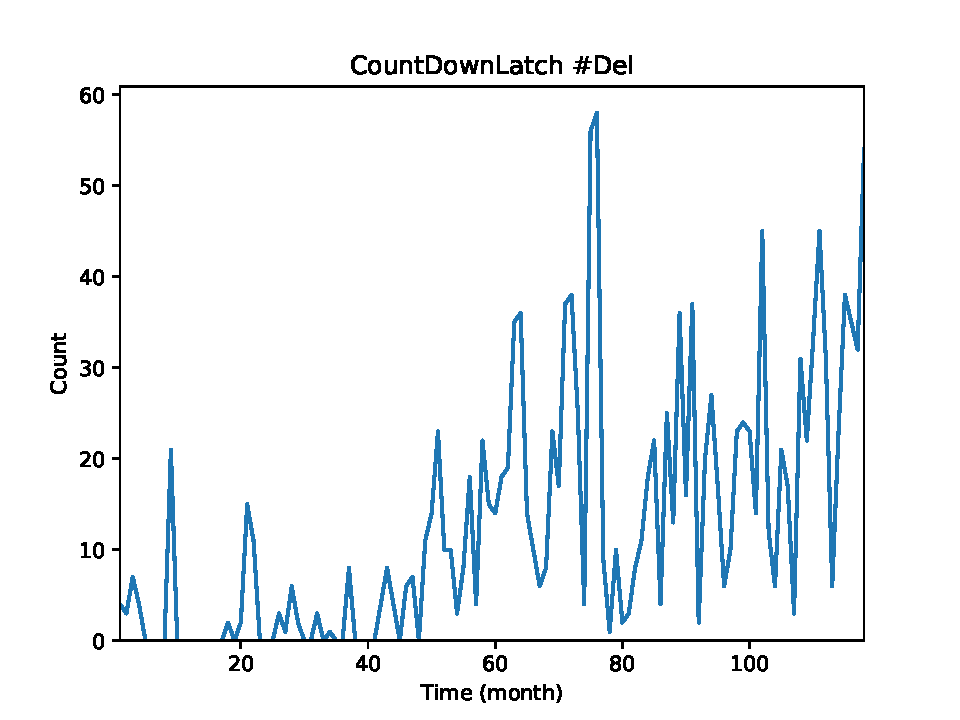
\includegraphics[height=1.5in]{CountDownLatchMinus}
%	\caption{Removal of CountDownLatch}
%\end{figure}
Table~\ref{table:topapi} shows the top ten active parallel API classes in Java. Column ``class'' lists names of these classes. Column ``Occurrence'' lists their occurrences in our concurrency-related commits. Dig~\cite{conf/sigsoft/OkurD12} found that in C\#, 10\% of parallel API classes account for 90\% of API usages. We find that Java follows similar usages patterns as C\#. However, the distribution of Java is not as screwed as C\#. We find that the top \%10 classes account only for about 50\% of the total occurrences, while the bottom \%10 classes account for 0.36\%.

Based on their occurrences, we put the 53 classes into three categories such as \emph{high-frequency}, \emph{medium-frequency} and \emph{low-frequency}, and each category contains roughly the same number of classes. For each category, we further put its classes into three subcategories such as \emph{ascending}, \emph{descending} and \emph{hybrid}. Figure~\ref{figure:trend} shows the results. The percent in each chart is calculated from the classes with the corresponding trend to the total classes. Although most classes are in the hybrid trend, we notice that in the high-frequent category, 15.1\% of classes are in the ascending subcategory. The trend can indicate that some popular parallel API classes are becoming more popular.

In summary, we find that Java parallel API classes follow a similar distribution as C\#, but the distribution is less screwed. However, the trends indicate that the distribution can become more like C\#, since popular ones are becoming more popular.

%Figure (a) shows an example of ascending tendency. It is \CodeIn{CountDownLatch}. We are not meaning it is in a strict ascending order. Its overall tendency is rising. Figure (b) shows an example of descending tendency. It is \CodeIn{LinkedTransferQueue}. However, most charts are like figure (c). They are fluctuating without certain ascending or descending tendency. We divide the classes into 3 parts equally and show one class of each part.

% There are 13 ascending charts, 4 descending charts and 36 hybrid charts.

%We write a program to count and analyze concurrent programming classes usage. Table IV shows top 10 classes added and deleted in the history. Some classes are both active in the added and the deleted column like AtomicInteger and CountDownLatch. This is not surprising because a deletion of class does not mean this class is abandoned. This also indicates this class is active. An interesting observation is that deletions appear more than addition.

%We draw line for addition and removal of each class. Figure 3 and figure 4 show examples. We can see that both numbers of addition and removal increase as a whole as time passing by. This indicates that this class is attracting developers' attention.

\subsection{RQ4. The correlations between total commits and concurrency-related commits.}
\label{sec:result:correlation}




Figure~\ref{fig:confidence} shows our results. Each label denotes a project, and has two associated figures. In particular, the upper figure denotes total commits and concurrency-related commits in the interval of months. Its horizontal axis denotes time, and its vertical axis denotes number of commits. Its blue curve denotes total commits, and its yellow curve denotes concurrency-related commits. We find that the curves of total commits and concurrency-related commits are not quite similar. However, the Spearman's rank correlation coefficient shows that in the five out of six projects, the two sets of values are correlated. One exception is Cassandra, where the correlation value is at the border (0.094).

In the lower figures, we calculate the percents from total commits to concurrency-related commits. Although the two sets of data are correlated, we find that their percents are inconstant. In total, about 20\% of total commits are related to concurrency. However, if we make predication based on the percents, the prediction can be unreliable.

In summary, we find that at a coarser granularity, the correlation between total commits and concurrency-related commits still exists, but the correlation becomes less significant.
%\zhong{Delete the following confidences, since you add them in Figure~\ref{fig:confidence} already}.

%\zhong{Introduce your null hypothesis. Introduce how to decide to reject a null hypothesis. That is, introduce how you determine two curves are coefficient.}.



%The coefficients are 0.094 for Cassandra, 0.844 for Flink, 0.868 for Hadoop, 0.896 for Lucene, 0.910 for Netty and 0.745 for Tomcat. Our result is consistent with Gu's result except one project.

%\zhong{Explain whether your results are consistent with Shan Lu or not. }

\subsection{Threats to Validity}

The threats to internal validity include that our tool can omit some concurrency commits. Due to various issues, our tool can fail to identify all concurrency commits. To reduce the threat, we employ both the query-based search and a classifier in our study. The threat could be further reduced by more advanced identification techniques. The threats to internal validity also include obsolete commits. With the rapid development of software, such commits may present obsolete or even wrong usages. To reduce the threat, in our study, we prefer to recent commits. The threats to external validity include our selected projects and programming language. The number of the projects we select is small compared to the huge amount of open-source projects. The threat could be reduced by introducing more projects and languages in future work.

